\documentclass{article}

\usepackage{graphicx}
\usepackage[hidelinks]{hyperref}
\usepackage{geometry}
\usepackage{amsmath}
\usepackage{listings}
\usepackage{wrapfig}

\geometry{
 a4paper,
 left=20mm,
 right=20mm,
 top=20mm,
 bottom=25mm,
}

\begin{document}

\begin{titlepage}
\begin{center}
\vspace*{1cm}
            
\Huge
\textbf{Assignment 1}
            
\vspace{1cm}

\Large
\text{Tuesday, September 17, 2024}

\vspace{2cm}

\text{\texttt{Wayne Rudnick}} \\
\text{\texttt{Jeremy Middleman}} \\
\text{\texttt{Brian High}} \\
\text{\texttt{Andrei Phelps}} \\
\text{\texttt{Thomas Hynes}} \\

\vspace{2cm}

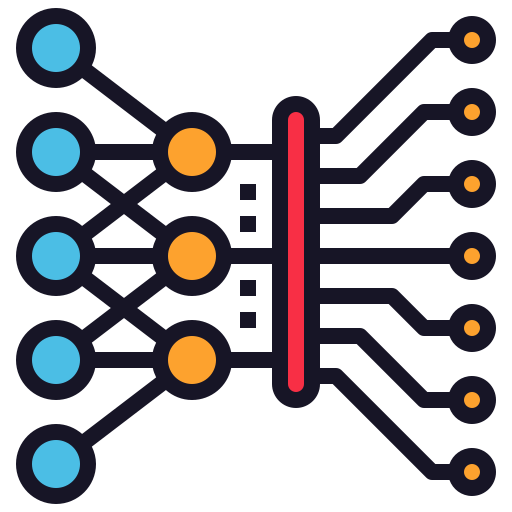
\includegraphics[scale=0.25]{../figs/icon.png}\\[0.5cm]

\vspace{9cm}

\textbf{CS 491/591: Neural Networks} \\

\end{center}
\end{titlepage}

\newpage
\section{How to Run the Program}
You can run the program by executing the main file using the python command.
\begin{verbatim}
    python main.py
\end{verbatim}
\section{Code Organization}
We structured our project into two files: main and perception. The main file is responsible for generating the training and test datasets, training the model, and adjusting model parameters. It also uses Matplotlib to visualize the training and testing results. The Perception file contains the Perception class and its member functions. After running the code, the command line displays the number of misclassified samples. \\ \\
\textbf{Note}: Case 3 was not plotted because it is 4 dimensional data and not part of the assignment instructions. 

\section{Methodology and Model Evaluation}
We implemented both the perceptron learning algorithm and gradient descent variants of the perceptron based on the material presented in lecture. To evaluate the performance of these two models under the conditions specified in the assignment, we conducted multiple tests, adjusting the learning rate and the number of epochs.

Additionally, we decided to plot both the training and test data to evaluate how well our model's parameters were tuned for the test cases. This comparison allowed us to assess the model's performance on the training data versus the test data. According to the Perceptron Convergence Theorem, a perceptron will perfectly classify a linearly separable dataset given sufficient epochs and the use of the perceptron learning algorithm. Therefore, if we observed the perceptron failing to perfectly classify the training data, it indicated that parameter adjustments were necessary.

\section{Perceptron}

\subsection{Perceptron Learning Algorithm}

For parts 1-3 of the assignment, we chose to run our test with 10 epochs at a learning rate of 0.1.  Due to the relatively simple nature of this test case, we wanted to see how the model performed with parameters that we thought were conservative. Even with this relatively low number of epochs, the perceptron effectively classified the data. Our post-training perceptron model correctly classified all test samples for Case #1 and missed 5 test samples for case #2. This near 100\% accuracy in both cases is likely because the data is completely linearly separable. Had the data been less linearly separable, we expect that the model would not have been as accurate.


\subsubsection{Test 1}

\begin{center}
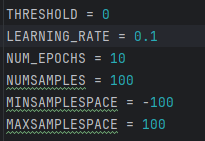
\includegraphics[scale=0.75]{../figs/T1.1.png} \\
\caption{Model Parameters}
\end{center}

\begin{center}
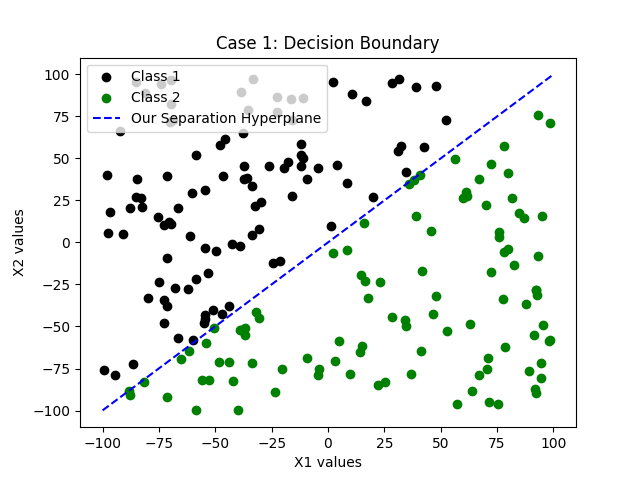
\includegraphics[scale=0.75]{../figs/T1.2.png} \\
\end{center}

\begin{center}
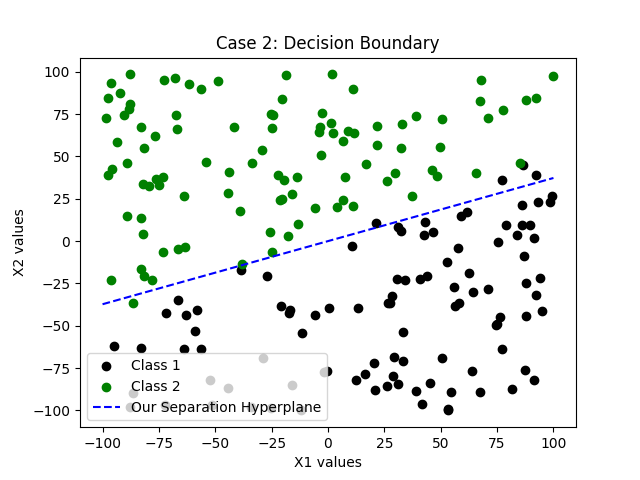
\includegraphics[scale=0.75]{../figs/T1.3.png} \\
\end{center}

\begin{center}
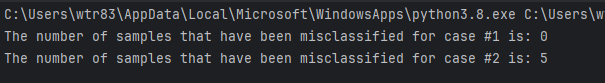
\includegraphics[scale=0.75]{../figs/T1.4.png} \\
\end{center}

The model performs well under with what determined to be reasonable values. 
\subsubsection{Test 2}
We increased the learning rate by 100-fold to see if we could cause the model to exhibit unstable behavior.

\begin{center}
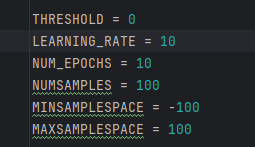
\includegraphics[scale=0.75]{../figs/T2.1.png} \\
\caption{Model Parameters}
\end{center}

\begin{center}
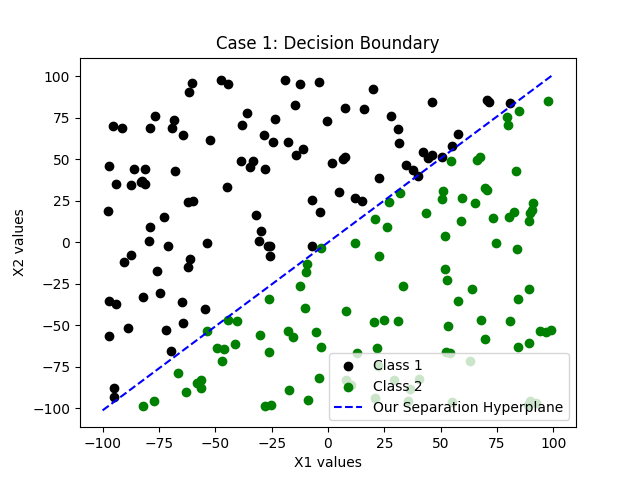
\includegraphics[scale=0.75]{../figs/T2.2.png} \\
\end{center}

\begin{center}
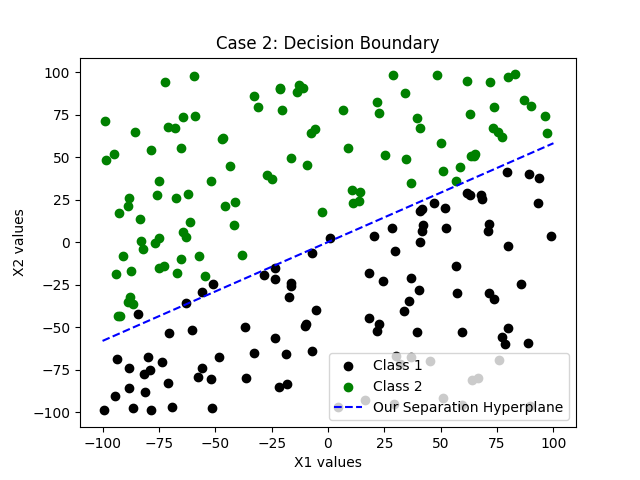
\includegraphics[scale=0.75]{../figs/T2.3.png} \\
\end{center}

\begin{center}
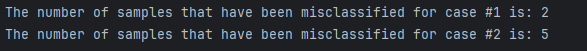
\includegraphics[scale=0.75]{../figs/T2.4.png} \\
\end{center}


With these parameters, the model's performance was comparable to that of Test 1.

\subsubsection{Test 3}

For our additional test with 10,000 samples, we observed a very defining line between class 1 and class 2. We wanted to include this test in our document because we believe it does a good job of showing how well the separation hyperplane is positioned when it has lots of training data. In this example, the hyperplane only has a mistake rate of approximately 1\%.

\begin{center}
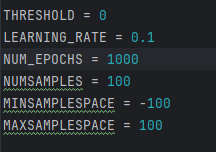
\includegraphics[scale=0.75]{../figs/T3.1.png} \\
\caption{Model Parameters}
\end{center}

\begin{center}
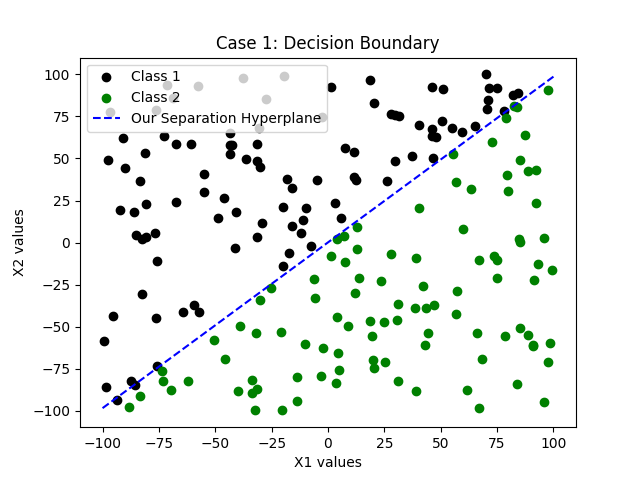
\includegraphics[scale=0.75]{../figs/T3.2.png} \\
\end{center}

\begin{center}
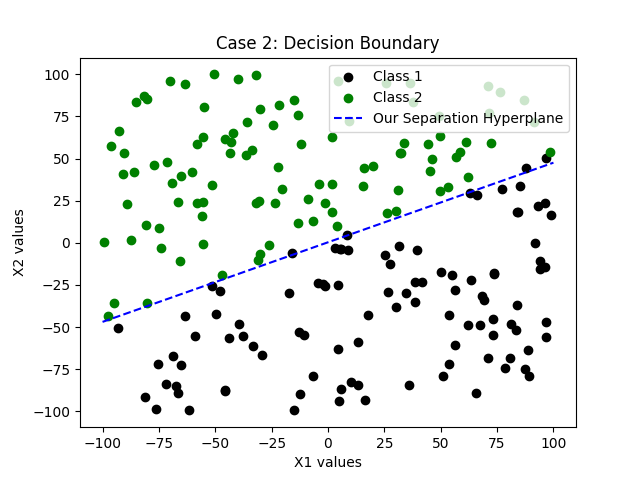
\includegraphics[scale=0.75]{../figs/T3.3.png} \\
\end{center}

\begin{center}
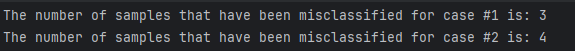
\includegraphics[scale=0.75]{../figs/T3.4.png} \\
\end{center}

\subsubsection{Test 4}

\begin{center}
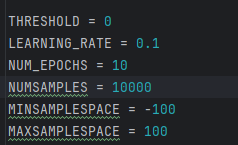
\includegraphics[scale=0.75]{../figs/T4.1.png} \\
\caption{Model Parameters}
\end{center}

\begin{center}
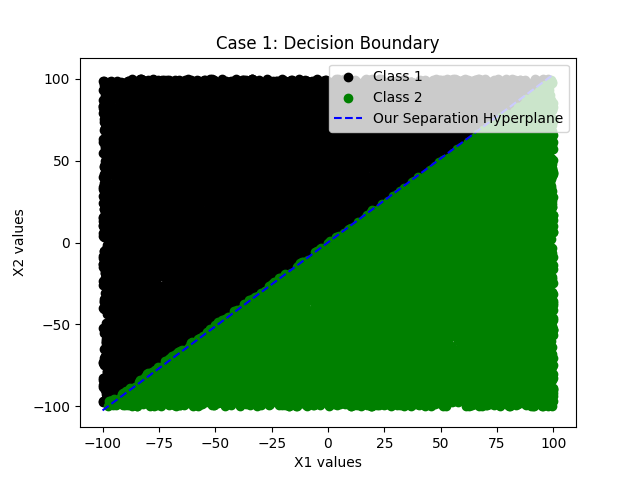
\includegraphics[scale=0.75]{../figs/T4.2.png} \\
\end{center}

\begin{center}
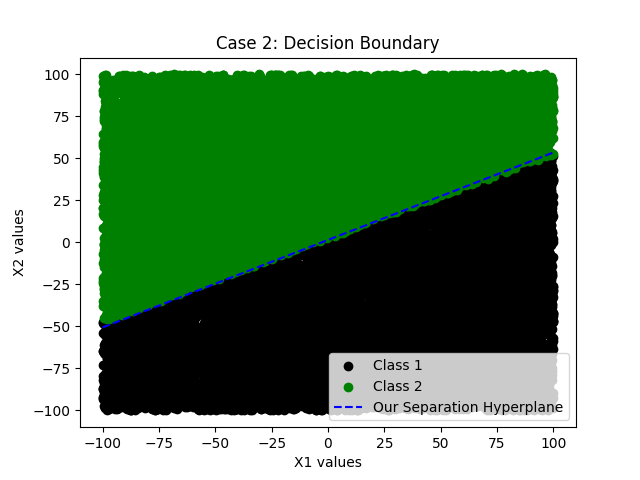
\includegraphics[scale=0.75]{../figs/T4.3.png} \\
\end{center}

\begin{center}
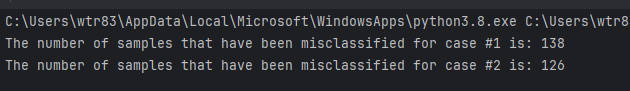
\includegraphics[scale=0.75]{../figs/T4.4.png} \\
\end{center}

\subsection{Gradient Descent}

\subsubsection{Test 5}

Test 5 has the same set up as test one to act as a comparison to perceptron learning algorithm, however this time using the gradient descent (GD) algorithm. The GD algorithm equalled or improved upon the accuracy of the perceptron learning algorithm as reflected in the data for case 1 (case 3 not pictured, but visible if the program is run). However it wasn't a massive improvement. In one run of the program in case 3, 13 samples were misclassified in the training data using the PLA while two were misclasssified with the GD algorithm. The PLA is still capable of separating the data even with higher dimensionality sample data. However the more dimensions that are added or the less linearly-separable that the data becomes, we may predict that there would be a significant decrease in accuracy for the PLA but not nearly as great of a decrease in the GD algorithm. This is because of the advantages of the GD algorithm over PLA, namely that the GD loss equation factors in the overall inaccuracy of the sample instead of just whether the sample was classified correctly or not.
\begin{center}
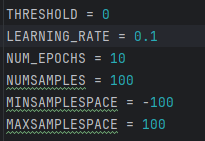
\includegraphics[scale=0.75]{../figs/T1.1.png} \\
\caption{Model Parameters}
\end{center}

\begin{center}
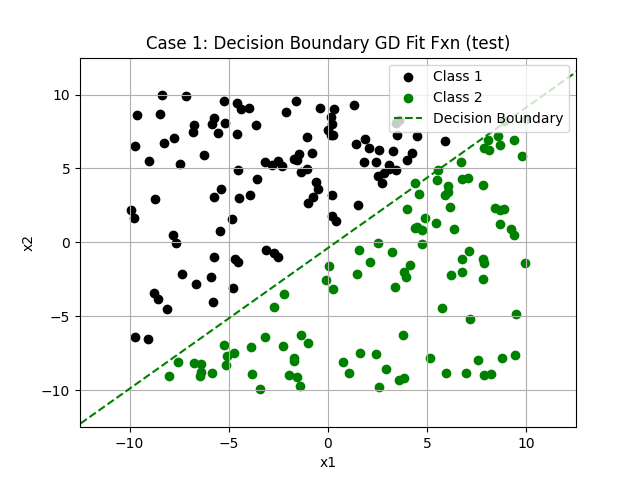
\includegraphics[scale=0.75]{../figs/T5.2.png} \\
\end{center}

\begin{center}

\includegraphics[scale=0.75]{../figs/T5.4.png} \\
\end{center}

\begin{center}
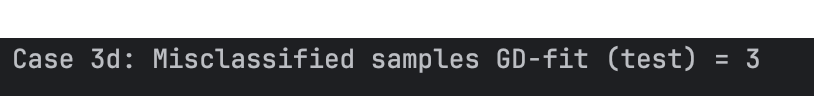
\includegraphics[scale=0.75]{../figs/T5.3.png} \\
\end{center}

\subsubsection{Test 6}

Again increasing the learning rate did not effect the stability of the model in this case.

\begin{center}
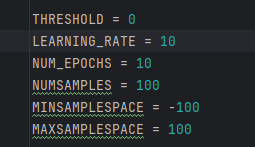
\includegraphics[scale=0.75]{../figs/T2.1.png} \\
\caption{Model Parameters}
\end{center}

\begin{center}
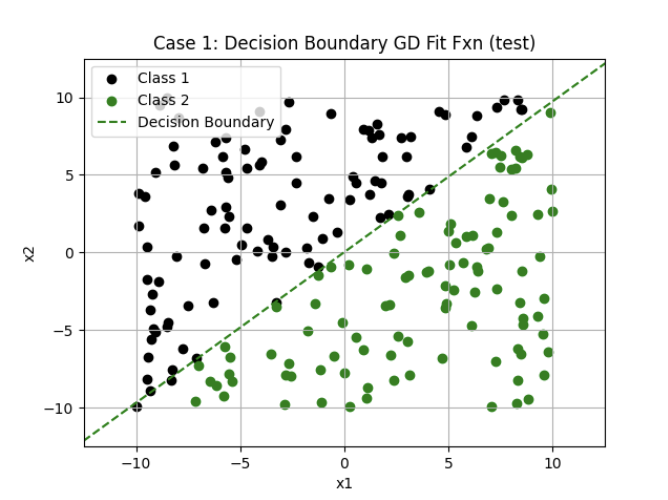
\includegraphics[scale=0.75]{../figs/T6.1.png} \\
\end{center}

\begin{center}

\includegraphics[scale=0.75]{../figs/T6.2.png} \\
\end{center}

\begin{center}

\includegraphics[scale=0.75]{../figs/T6.3.png} \\
\end{center}

\subsubsection{Test 7}

With a large number of epochs the model performs very well.
\begin{center}
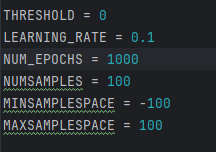
\includegraphics[scale=0.75]{../figs/T3.1.png} \\
\caption{Model Parameters}
\end{center}

\begin{center}
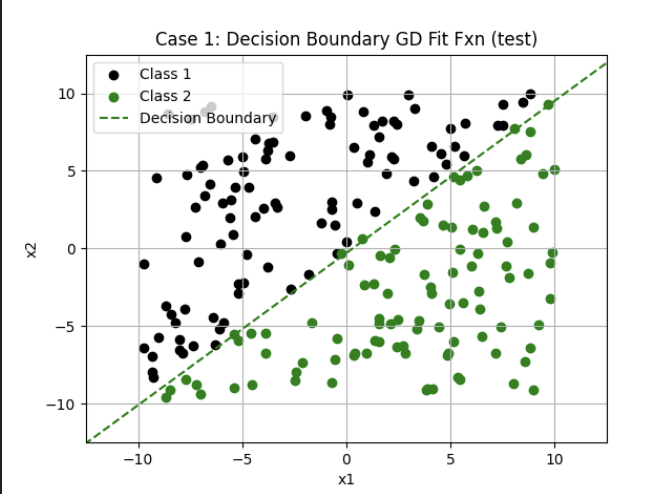
\includegraphics[scale=0.75]{../figs/T7.1.png} \\
\end{center}

\begin{center}

\includegraphics[scale=0.75]{../figs/T7.2.png} \\
\end{center}

\begin{center}

\includegraphics[scale=0.75]{../figs/T7.3.png} \\
\end{center}

\subsubsection{Test 8}

\begin{center}
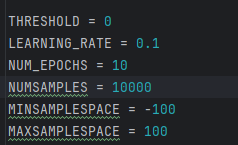
\includegraphics[scale=0.75]{../figs/T4.1.png} \\
\caption{Model Parameters}
\end{center}

\begin{center}
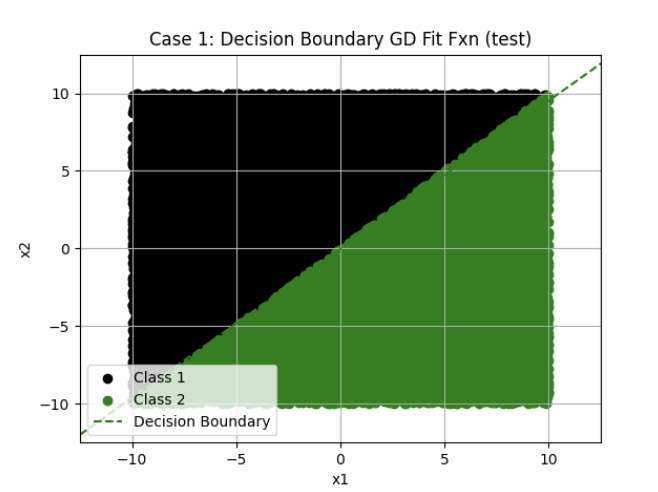
\includegraphics[scale=0.75]{../figs/T8.1.png} \\
\end{center}

\begin{center}

\includegraphics[scale=0.75]{../figs/T8.2.png} \\
\end{center}

\begin{center}

\includegraphics[scale=0.75]{../figs/T8.3.png} \\
\end{center}

\section{Individual Contributions}

\subsection{Wayne Rudnick}
\begin{itemize}
    \item[1)] Initialized the GitHub repository and guided the team in starting the project.
    \item[2)] Developed the perceptron class, including the fit function, test cases, and training data. Plotted the separation hyperplane and analyzed misclassified samples.
    \item[3)] Assisted with parts 4 and 5 by adapting earlier code, providing guidance, and generating additional tests and graphs.
\end{itemize}

\subsection{Jeremy Middleman}
\begin{itemize}
    \item[1)] Helped with part 5 of the assignment, including writing sample generation, sample testing, and plot generation.
    \item[2)] Helped write the report, specifically the section on gradient descent.
\end{itemize}

\subsection{Brian High}
\begin{itemize}
    \item[1)] Worked on the document.
    \item[2)] Helped with Gradient Decent.
    \item[3)] Helped with test cases.
\end{itemize}

\subsection{Andrei Phelps}
\begin{itemize}
    \item[1)] Contributed to the development of parts 4 and 5 of the code.
    \item[2)] Created the LaTeX document and provided support in writing the final report.
    \item[3)] Assisted in creating test cases and refining the code and report for submission.
\end{itemize}

\subsection{Thomas Hynes}
\begin{itemize}
    \item[1)] Added comments in code to enhance readability.
    \item[2)] Assisted in finalizing the report.
\end{itemize}

\end{document}
